%%%%%%%%%%%%%%%%%%%%%%%%%%%%%%%%%%%%%%%%%%
% Engineering problems / LaTeX Template
%		Semester 5
%		Institut d'Optique Graduate School
%%%%%%%%%%%%%%%%%%%%%%%%%%%%%%%%%%%%%%%%%%
%	5N-ONIP-Block1	/ Python for Science
%%%%%%%%%%%%%%%%%%%%%%%%%%%%%%%%%%%%%%%%%%
%
% Created by:
%	Julien VILLEMEJANE - 25/sep/2024
% Modified by:
%	
%
%%%%%%%%%%%%%%%%%%%%%%%%%%%%%%%%%%%%%%%%%%
% Professional Newsletter Template
% LaTeX Template
% Version 1.0 (09/03/14)
%
% Created by:
% Bob Kerstetter (https://www.tug.org/texshowcase/) and extensively modified by:
% Vel (vel@latextemplates.com)
% 
% This template has been downloaded from:
% http://www.LaTeXTemplates.com
%
% License:
% CC BY-NC-SA 3.0 (http://creativecommons.org/licenses/by-nc-sa/3.0/)
%
%%%%%%%%%%%%%%%%%%%%%%%%%%%%%%%%%%%%%%%%%

\documentclass[10pt]{article} % The default font size is 10pt; 11pt and 12pt are alternatives

\input{../../../../../_assets/latex/5N_ONIP_structure.tex} % Include the document which specifies all packages and structural customizations for this template
\usepackage{amsmath}
\usepackage{schemabloc}

%----------------------------------------------------------------------------------------
%	DOCUMENT INFORMATIONS
%----------------------------------------------------------------------------------------
\def\module{Opto-Electronique}
\def\submodule{OptoElec}
\def\moduleSmall{5N-027-SCI / OE}
\def\year{2024-2025}
\def\problem{TD Systèmes et Signaux}
\def\problemName{OptoElec \& ONIP-1 / TD Systèmes et Signaux}

\def\validation{}

\def\scheduleCM{0}
\def\scheduleTD{0}
\def\scheduleTDcomputer{2}
\def\scheduleTP{0}

\def\workingTeam{Par binôme}

\def\workingSpecial{}

\def\keywords{Systèmes asservis;ALI;FFT}


\begin{document}
%----------------------------------------------------------------------------------------
%	HEADER IMAGE
%----------------------------------------------------------------------------------------

\begin{figure}[H]
\centering\includegraphics[width=0.3\linewidth]{../../../../../_assets/latex/logo_iogs.png}
\end{figure}

%----------------------------------------------------------------------------------------
%	MAIN BODY - FIRST PAGE
%----------------------------------------------------------------------------------------
%
\hypertarget{context}{\heading{\huge \problemName}{6pt}} % \hypertarget provides a label to reference using \hyperlink{label}{link text}

%-----------------------------------
\centerline {\rule{.70\linewidth}{.25pt}} % Horizontal line
\begin{center}
\textsc{\large Séance 1 / Systèmes asservis}
\end{center}
\centerline {\rule{.70\linewidth}{.25pt}} % Horizontal line
%-----------------------------------

%-----------------------------------
\textbf{Exercice 1 / Modélisation numérique d'un système / ALI}

Soit un système $A(j\omega)$ de type passe-bas, d'ordre 1, de gain statique $A_0$ et de pulsation de coupure $w_0$.

\begin{enumerate}
	\item Donner la fonction de transfert de ce système.
	\item A l'aide de la bibliothèque \textbf{control} sous Python, définir la fonction de transfert de ce système à l'aide de la fonction \textsl{tf}.
	\item Tracer la \textbf{réponse en fréquence} de ce système à l'aide de la fonction \textsl{bode\_plot}.
	\item Tracer la \textbf{réponse indicielle} à l'aide de la fonction \textsl{step\_response}, puis \textbf{impulsionnelle} à l'aide de la fonction \textsl{impulse\_response}.
	\item Calculer et afficher la \textbf{transformée de Fourier} de la réponse impulsionnelle. Que pouvez-vous en conclure ?
	
\end{enumerate}

Applications Numériques : $A_0 = 10^5$, $f_0 = 30\operatorname{Hz}$.

\centerline {\rule{.70\linewidth}{.25pt}} % Horizontal line

Fonction de transfert :

$$A(j\omega) = \frac{A_0}{1 + j \cdot \frac{\omega}{\omega_0}}$$

Représentation sous forme d'un schéma bloc :

\begin{center}
\Large
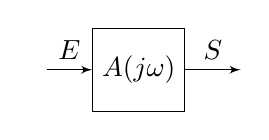
\begin{tikzpicture}
	\sbEntree{E}
		\sbBloc{sysA}{$A(j\omega)$}{E}
    \sbSortie{S}{sysA}
    \sbRelier[$E$]{E}{sysA}
    \sbRelier[$S$]{sysA}{S}
\end{tikzpicture}
\end{center}

Définition du système avec la bibliothèque \textbf{control} :

\begin{lstlisting}[language=Python]
import control as ct

A0 = 1e5
f0 = 30
w0 = 2 * np.pi * f0

num_A = [A0]
den_A = [1/w0, 1]
sys_A = ct.tf(num_A, den_A)
\end{lstlisting}

\newpage
\textbf{Diagramme de Bode du système} :

\begin{lstlisting}[language=Python]
# Bode diagram
w = np.logspace(1, 6, 101)
ct.bode_plot([sys_A], w, name='A')
plt.show()
\end{lstlisting}

\includegraphics{exo1_1.png}

\newpage
\textbf{Réponse indicielle du système} :

\begin{lstlisting}[language=Python]
time = np.arange(0, 0.1, 0.0001)

T, yout = ct.step_response(sys_A, time)
plt.figure()
plt.plot(T, yout)
plt.xlabel("time (s)")
plt.ylabel("Step Response")
plt.grid()
\end{lstlisting}

\includegraphics{exo1_2.png}


\newpage
\textbf{Réponse impulsionnelle du système} :

\begin{lstlisting}[language=Python]
T, yout = ct.impulse_response(sys_A, time)
plt.figure()
plt.plot(T, yout)
plt.xlabel("time (s)")
plt.ylabel("Step Response")
plt.grid()
\end{lstlisting}

\includegraphics{exo1_3.png}


\newpage
\textbf{Transformée de Fourier discrète} de la réponse impulsionnelle du système :

\begin{lstlisting}[language=Python]
tf_yout = np.fft.fft(yout)
tf_yout = tf_yout / len(tf_yout)
plt.figure()
plt.semilogx(np.abs(tf_yout[:len(tf_yout)//2]))
plt.xlabel("Freq")
plt.ylabel("Step Response TF")
plt.grid()
plt.show()
\end{lstlisting}

\includegraphics{exo1_4.png}

\newpage
\centerline {\rule{.70\linewidth}{.25pt}} % Horizontal line
%-----------------------------------
\textbf{Exercice 2 / Rebouclage d'un système - Système asservi / ALI en régime "linéaire"}

Il est possible de reboucler un système à l'aide d'un autre système. On parle alors d'un système asservi. 

On prendra ici le système $A$ pour la boucle d'action et un système $B(j\omega) = 1 / K$, où $K$ est une constante, comme système de contre-réaction.

\begin{enumerate}
	\item Tracer le \textbf{schéma bloc} de ce système puis donner la \textbf{fonction de transfert} de ce système.
	\item Que vaut le \textbf{produit} du gain statique par la fréquence de coupure de ce système ? Comparer cette valeur à celui du système $A$. Que pouvez-vous en conclure ?	
	
	\medskip	
	
	\item Définir la \textbf{fonction de transfert} du système $B$ à l'aide de la fonction \textsl{tf}.
	\item Définir un système $C$ qui est le système complet avec la rétro-action, à l'aide de la fonction \textsl{feedback}.
	\item Tracer la \textbf{réponse en fréquence} des systèmes $A$ et $C$ à l'aide de la fonction \textsl{bode\_plot} sur un même graphique.
	\item Tracer la \textbf{réponse indicielle} des systèmes $A$ et $C$ à l'aide de la fonction \textsl{step\_response} sur un même graphique.
\end{enumerate}

Applications Numériques : $A_0 = 10^5$, $f_0 = 30\operatorname{Hz}$ et $K = 1$ puis $K = 10$.

\centerline {\rule{.70\linewidth}{.25pt}} % Horizontal line

\textbf{Schéma bloc du système} :

\begin{center}
\Large
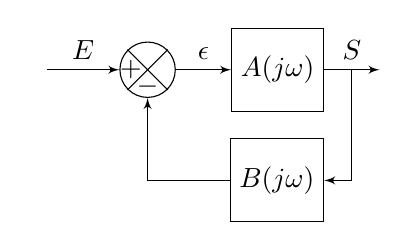
\begin{tikzpicture}
\sbEntree{E}
	\sbComp{comp}{E}
	\sbRelier[$E$]{E}{comp}
\sbBloc{sysA}{$A(j\omega)$}{comp}
	\sbRelier[$\epsilon$]{comp}{sysA}
\sbSortie{S}{sysA}
	\sbRelier[$S$]{sysA}{S}
\sbDecaleNoeudy[4]{S}{U}
\sbBlocr{sysB}{$B(j\omega)$}{U}
\sbRelieryx{sysA-S}{sysB}
\sbRelierxy[]{sysB}{comp}

%\sbBloc{sys}{Système}{reg}
%\sbRelier[u]{reg}{sys}
%\sbRelier[$S_1$]{sys}{S}
%\sbRelieryx{sys-S}{cap}
%\sbRelierxy[m]{cap}{comp}
\end{tikzpicture}
\end{center}

\textbf{Fonction de transfert du système} :

On peut calculer

$$\epsilon = E - B(j\omega) \cdot S$$

$$S = A(j\omega) \cdot \epsilon$$

En regroupant ces expressions on obtient :

$$\frac{S}{E} = \frac{A(j\omega)}{1 + A(j\omega) \cdot B(j\omega)}$$

En remplaçant $A(j\omega)$ et $B(j\omega)$ par leurs expressions respectives, on obtient : 

{\Large
$$H_{BF} = \frac{S}{E} = \frac{A_0}{\frac{A_0}{K} + 1} \cdot \frac{1}{1 + \frac{j\omega}{\omega_0 \cdot (1 + \frac{A_0}{K})}}$$
}

On peut alors identifier le gain statique et la fréquence de coupure de ce nouveau système :

$H_{BF0} = \frac{A_0}{\frac{A_0}{K} + 1}$ et $\omega_{BF0} = \omega_0 \cdot (1 + \frac{A_0}{K})$

Le produit des deux donne : $H_{BF0} \cdot \omega_{BF0} = A_0 \cdot \omega_0 = cte$ 

\newpage

\textbf{Définition des systèmes B et C} :

\begin{lstlisting}[language=Python]
K = 10
sys_B = ct.tf([1],[K], name='B')

sys_C = ct.feedback(sys_A, sys_B, name='C')
\end{lstlisting}

\textbf{Diagramme de Bode des systèmes A et C} :

\begin{lstlisting}[language=Python]
w = np.logspace(1, 8, 101)
ct.bode_plot([sys_A, sys_C], w)
plt.show()
\end{lstlisting}

\includegraphics{exo2_1.png}

\textbf{Réponse indicielle des systèmes A et C} :

\begin{lstlisting}[language=Python]
time = np.arange(0, 0.1, 0.000001)

T, yout_A = ct.step_response(sys_A, time)
T, yout_C = ct.step_response(sys_C, time)
plt.figure()
plt.plot(T, yout_A, label='A')
plt.plot(T, 1e4*yout_C, label='C (*1e4)')
plt.xlabel("time (s)")
plt.ylabel("Step Response")
plt.grid()
plt.show()
\end{lstlisting}

\includegraphics{exo2_2.png}

\includegraphics{exo2_3.png}




\newpage
\centerline {\rule{.70\linewidth}{.25pt}} % Horizontal line
%-----------------------------------
\textbf{Exercice 3 / Système du second ordre}

On se propose de simuler un système du second ordre dont la fonction de transfert peut être mise sous la forme suivante :

$$H(j\omega) = \frac{A_0 \cdot (\frac{j \cdot \omega}{\omega_0})^2}{1 + 2 \cdot m \cdot \frac{j \cdot \omega}{\omega_0} + (\frac{j \cdot \omega}{\omega_0})^2}$$

\begin{enumerate}
	\item Définir ce système.
	\item Tracer la réponse en fréquence de ce système pour $m = [0.1, 0.5, 0.7, 1.0, 2]$ sur un même graphique.
	\item Tracer la réponse indicielle de ce système pour $m = [0.1, 0.5, 0.7, 1.0, 2]$ sur un même graphique.
\end{enumerate}

Applications Numériques : $A_0 = 10$, $f_0 = 1000\operatorname{Hz}$.


\centerline {\rule{.70\linewidth}{.25pt}} % Horizontal line

\begin{lstlisting}[language=Python]
import control as ct
import numpy as np
from matplotlib import pyplot as plt

# Parameters of the system
A0 = 10    # V/V
f0 = 1000	    # Hz
w0 = 2*np.pi*f0   # rd/s
m = [0.1, 0.5, 0.707, 1, 2]
m_n = ['0,1', '0,5', '0,707', '1', '2']

sys_H = []

for i, mm in enumerate(m):
    num = [A0/(w0**2), 0, 0]
    den = [1/w0**2, 2*float(mm)/w0, 1]
    nameH = f'H{i} / m={m_n[i]}'
    sys = ct.tf(num, den, name=nameH)
    sys_H.append(sys)

# Bode diagram
w = np.logspace(2, 6, 101)
ct.bode_plot(sys_H, w)
plt.legend()
\end{lstlisting}

\includegraphics{exo3_1.png}

\begin{lstlisting}[language=Python]
# Step Response
time = np.arange(0, 0.01, 0.00001)
plt.figure()
for i, sys in enumerate(sys_H):
    T, yout_H = ct.step_response(sys, time)
    plt.plot(T, yout_H, label=f'H{i}')
plt.xlabel("time (s)")
plt.ylabel("Step Response")
plt.grid()
plt.legend()
plt.show()
\end{lstlisting}

\includegraphics{exo3_2.png}


\newpage
%-----------------------------------
\centerline {\rule{.70\linewidth}{.25pt}} % Horizontal line
\begin{center}
\textsc{\large Bibliothèque CONTROL}
\end{center}
\centerline {\rule{.70\linewidth}{.25pt}} % Horizontal line
%-----------------------------------

Plus d'aide sur la bibliothèque \textbf{control} : \href{https://python-control.readthedocs.io/en/0.10.1/}{https://python-control.readthedocs.io/en/0.10.1/}

Pour importer la bibliothèque \textbf{control} :  
\begin{lstlisting}[language=python]
import control as ct
\end{lstlisting}

%-----------------------------------
\centerline {\rule{.70\linewidth}{.25pt}} % Horizontal line
\textbf{Définir un système}

La \textbf{définition d'un système} par l'intermédiaire d'une fonction de transfert se fait à l'aide de la fonction \textsl{tf} :

\begin{lstlisting}[language=python]
# System with a transfert function : (3s + 4) / (6s^2 + 5s + 4).
num = [3, 4]
den = [6, 5, 4]
sys1 = ct.tf(num, den)
\end{lstlisting}

%-----------------------------------
\centerline {\rule{.70\linewidth}{.25pt}} % Horizontal line
\textbf{Tracer la réponse en fréquence d'un système}

Il est possible de tracer la réponse en fréquence d'un système à l'aide de la fonction \textsl{bode\_plot} : 

\begin{lstlisting}[language=python]
ct.bode_plot(sys1)
plt.show()
\end{lstlisting}

\textit{Attention : cette fonction se base sur la bibliothèque Pyplot de Matplotlib. Il est indispensable de l'importer et de faire appel à la fonction show() pour visualiser les graphiques.}

Il est également possible de passer une liste de système en argument de la fonction \textsl{bode\_plot} afin de comparer plusieurs systèmes entre eux.

%-----------------------------------
\centerline {\rule{.70\linewidth}{.25pt}} % Horizontal line
\textbf{Tracer la réponse indicielle d'un système}

Il est possible de tracer la réponse à un échelon d'un système à l'aide de la fonction \textsl{step\_response} : 

\begin{lstlisting}[language=python]
time = np.arange(0, 0.1, 0.0001)
T, yout = ct.step_response(sys1, time)
\end{lstlisting}

Cette fonction renvoie deux vecteurs : un vecteur temps (\textsl{T}) et le signal de sortie de la réponse à l'échelon (\textsl{yout}). Le vecteur \textsl{time} n'est pas indispensable. S'il n'est pas fourni, il est automatiquement calculé par la fonction \textsl{step\_response}.

Pour pouvoir afficher le graphique associé, il est indispensable d'utiliser une bibliothèque graphique de type Pyplot de Matplotlib.

%-----------------------------------
\centerline {\rule{.70\linewidth}{.25pt}} % Horizontal line
\textbf{Tracer la réponse impulsionnelle d'un système}

Il est possible de tracer la réponse à une impulsion d'un système à l'aide de la fonction \textsl{impulse\_response} : 

\begin{lstlisting}[language=python]
time = np.arange(0, 0.1, 0.0001)
T, yout = ct.impulse_response(sys1, time)
\end{lstlisting}

Cette fonction renvoie le même type de données que \textsl{step\_response}


%-----------------------------------
\centerline {\rule{.70\linewidth}{.25pt}} % Horizontal line
\textbf{Reboucler un système}

Il est possible de reboucler un système par un autre système à l'aide de la fonction \textsl{feedback} : 

\begin{lstlisting}[language=python]
sys = ct.feedback(sys1, sys2)
\end{lstlisting}


\end{document} 